\chapter{Manifolds and surfaces}

\section{Sides of a surface}

\fxerror{I have not defined connected components of a filter.}

\begin{defn}
Let $\mu$ be an endofuncoid on a set~$U$.
\emph{Surface side} of a set~$T\subseteq\Ob\mu$ is a connected component
(regarding $\mu$) of the filter $(\rsupfun{\mu}T)\setminus T$.
\fxnote{$\mu$ is used twice in this definition. We may generalize
for two different funcoids instead.}
\end{defn}

Keep in mind that the above definition may work nicely if~$\mu$ is
a complete funcoid induced by a topological space.

\begin{example}
For an $\mathbb{R}^{n-1}$ subspace~$T$ of a~$\mathbb{R}^n$ ($n\geq 1$)
euclidean space and the complete funcoid~$\mu$ induced by the usual topology:
\begin{enumerate}
\item $T$~has exactly two surface sides.
\item The filter $\rsupfun{\mu}@\{a\} \setminus T$ (for every $a\in T$)
  has exactly two connected components.
\end{enumerate}
\end{example}

\begin{proof}
Without loss of generality assume that
\[ T=\setcond{(x_0,x_1,\dots,x_{n-2},0)}{
x_0,x_1,\dots,x_{n-2}\in\mathbb{R}};
\quad
a = (0,\dots,0). \]

We have
\[ \rsupfun{\mu}@\{a\} =
\left(\uparrow\setcond{v\in\mathbb{R}^n}{v_{n-1}>0}\sqcap\rsupfun{\mu}@\{a\}\right)
\sqcup
\left(\uparrow\setcond{v\in\mathbb{R}^n}{v_{n-1}<0}\sqcap\rsupfun{\mu}@\{a\}\right). \]

Let us prove that
$\uparrow\setcond{v\in\mathbb{R}^n}{v_{n-1}>0}\sqcap\rsupfun{\mu}@\{a\}$ and
$\uparrow\setcond{v\in\mathbb{R}^n}{v_{n-1}<0}\sqcap\rsupfun{\mu}@\{a\}$ are
connected components.

??
\end{proof}

\subsection{Special points}

We will start from the example of open $T=\setcond{(x,y,0)}{x^2+y^2<1}$
and closed $T=\setcond{(x,y,0)}{x^2+y^2\leq 1}$ disks in~$\mathbb{R}^3$.

\begin{xca}
Prove that open disk (in a usual 3-dimensional space) has two surface sides
and closed disk has one surface side.
\end{xca}

\section{Special points}

\begin{defn}
\emph{Surface cardinality} of a point~$a$ (an element of the set $\Ob\mu$) is
the cardinality of the set of connected components of the filter
$\rsupfun{\mu}\{a\}\setminus T$.
\end{defn}

\begin{defn}
\emph{Cardinality regular point} is a point~$a$, which has a neighborhood
($X\in\up\rsupfun{\mu}\{a\}$) such that all points~$x\in X\cap T$
are of the same surface cardinality as the point~$a$.

\emph{Cardinality special point} is a point which is not cardinality regular.
\end{defn}

\begin{defn}
\emph{Isomorphism regular point} is a point~$a$, which has a neighborhood
($X\in\up\rsupfun{\mu}\{a\}$) such that for all points~$x\in X\cap T$
the filter $\rsupfun{\mu}\{a\}$ is isomorphic
to~$\rsupfun{\mu}\{x\}$.

\emph{Cardinality special point} is a point which is not cardinality regular.
\end{defn}

\fxnote{Try to replace isomorphism~$f$ with some kind of filter embedding.}

Consider the dihedral angle~$T$ produced by two half-planes. Are the points of
intersection of the half-planes isomorphism-special? (They should not
be considered special. If they are special, this is a probably flaw in
the definition of isomorphism special.)

Consider union~$T$ of two intersecting lines on a plane. The intersection
may be considered as a special point, because it has more connected
components that the rest. We don't want to consider it special, however.
We can restrict to consider special only points which have less connected
components (rather than more) to correct this trouble. Also try to define
it with some kind of morphisms of filters instead of isomorphism as in
isomorphism-special.

\begin{xca}
Excluding special points (either cardinality or isomorphism) from closed disk
produces open disk.
\end{xca}

Consider the following two subsets of a plane:

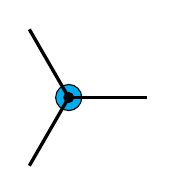
\begin{tikzpicture}
    \node at (0,0) [circle,draw,fill=cyan] (a) {};
    \fill (0,0) circle [radius=2pt,fill=black];
    \draw [very thick] (0,0) -- +(0:1cm);
    \draw [very thick] (0,0) -- +(120:1cm);
    \draw [very thick] (0,0) -- +(240:1cm);
\end{tikzpicture}

% \begin{tikzpicture}
%     \node[draw, fill=cyan, ellipse, text width=4pt] (a) {};
%     \draw (a) -- +(0:4cm);
%     \draw (a) -- +(120:4cm);
%     \draw (a) -- +(240:4cm);
% \end{tikzpicture}

Now define \emph{shift special points}.

Let $I$ be an interval on~$\mathbb{R}$ (containing zero?)

A point~$a$ is \emph{shift special} if there exists a transformation
(that is a continuous function $f:I\times\mu\to\mu$ such that:
\begin{enumerate}
  \item $f(0)$ is identity. \fxwarning{Is this condition needed?}
  \item for every sufficiently small~$\epsilon>0$ we have $f(\epsilon,a)\in T$;
  \item there is $\epsilon>0$ such that for every $0<\epsilon'<\epsilon$ we have
    $f(\epsilon')$ being not continuous at~$a$ regarding complete funcoid
    defined by the function $x\mapsto\rsupfun{\mu}\{x\}\setminus T$.
\end{enumerate}

We may consider to additonally require that every~$f(\epsilon)$ is isomorphism
of funcoids.

\begin{example}
$T$~is disk $\setcond{(x,y,0)}{x^2+y^2\leq 1}$. $f$~is the contraction
$(\epsilon,v)\mapsto\frac{1}{1+\epsilon}v$. $a=(1,0,0)$.

In the usual topology~$f$ is continuous. In
$x\mapsto\rsupfun{\mu}\{x\}\setminus T$ we have the function
$\epsilon\mapsto f(\epsilon)$ not continuous at zero.
So~$a$ is a shift special point.
\end{example}

\begin{proof}
$f (0) (v) = v$. Thus $\langle f (0) \rangle (\rsupfun{\mu} \{ a
\} \setminus T) = \rsupfun{\mu} \{ a \} \setminus T$ intersects
the plane $Z = 0$. But $f (0, a)$

??
\end{proof}

\begin{question}
Can we exclude real numbers from the play?
\end{question}

\begin{question}
How cardinality special points, isomorphism special points and shift
special points are related with each others?
\end{question}

\begin{question}
How the number of surface sides is related with usual surface sides for
manifolds?
\end{question}

Prove that $2$-manifold image which special points removed has the same number
of sides as the defined above.
